\chapter{cry if i want to} 
\label{sec:listing}
\lstset{style=6502Style}
Before the dawn of the three horsemen \textit{png}, \textit{gif} and \textit{jpg}, computer people were free to invent their 
own schemes for storing images. In 1991 technology was still
rudimentary enough that console and computer developers were largely pre-occupied with waging something resembling a \textit{Color War}. So
when Atari sat down to brew its own method of storing and representing image data one of its overriding concerns was \textit{how many
colours can we fit into this thing}.

The \textbf{CRY} file format is the result. 'Format' in this case is a slightly grandiose term for: here is a list of bytes in a file,
each pair of bytes in the list represents a color. Since a single byte has 256 possible values, two bytes has 65,536 possible values.
So welcome to our system that has a state-of-the-art 65,536 possible colours. Well, not quite. Let's see why.

\begin{definition}[Claw Says\index{Claw Says}]
\setlength{\intextsep}{0pt}%
\setlength{\columnsep}{3pt}%
\begin{wrapfigure}{l}{0.12\textwidth}
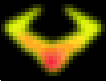
\includegraphics[width=\linewidth]{src/callout/claw.png} 
\end{wrapfigure}
\small
\textcolor{white}{
Good luck figuring out what CRY is an acryonym of. Maybe it refers to the three axes of the 'colour space': cyan, red, and yellow. 
Maybe it refers to the three components contained in each byte pair: color, radiance, and luminosity?
}
\end{definition}

In your innocence dear reader, you may expect that this color scheme is as simple as assigning a color to each of the possible values
and considering ourselves done for the day. But that is nowhere near complex enough to generate true job sastifaction. Instead, we must
declare something called a 'colour space' and declare co-ordinates along an X and Y axis. Even better, since this is not the 1980s
anymore, we ought to thinking in three dimensions and throw in a Z axis while we're at it.

\begin{figure}[H]
    \centering
    \begin{adjustbox}{width=7cm,center}
      \frame{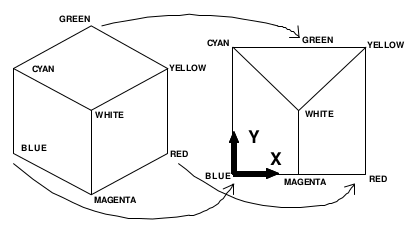
\includegraphics[width=12cm]{src/cry/axes.png}}%
    \end{adjustbox}
\caption{This kind of thing. This is what we want.}
\end{figure}

With just two bytes (or 16 bits) to work with we have to come up with a way that is suitably complicated for representing all our colours 
along so many co-ordinate axes. So let's imagine an 8x8x8 colour cube with something resembling white at its top corner and all the colours of
the spectrum radiating out of it.

\begin{figure}[H]
    \centering
    \begin{adjustbox}{width=7cm,center}
      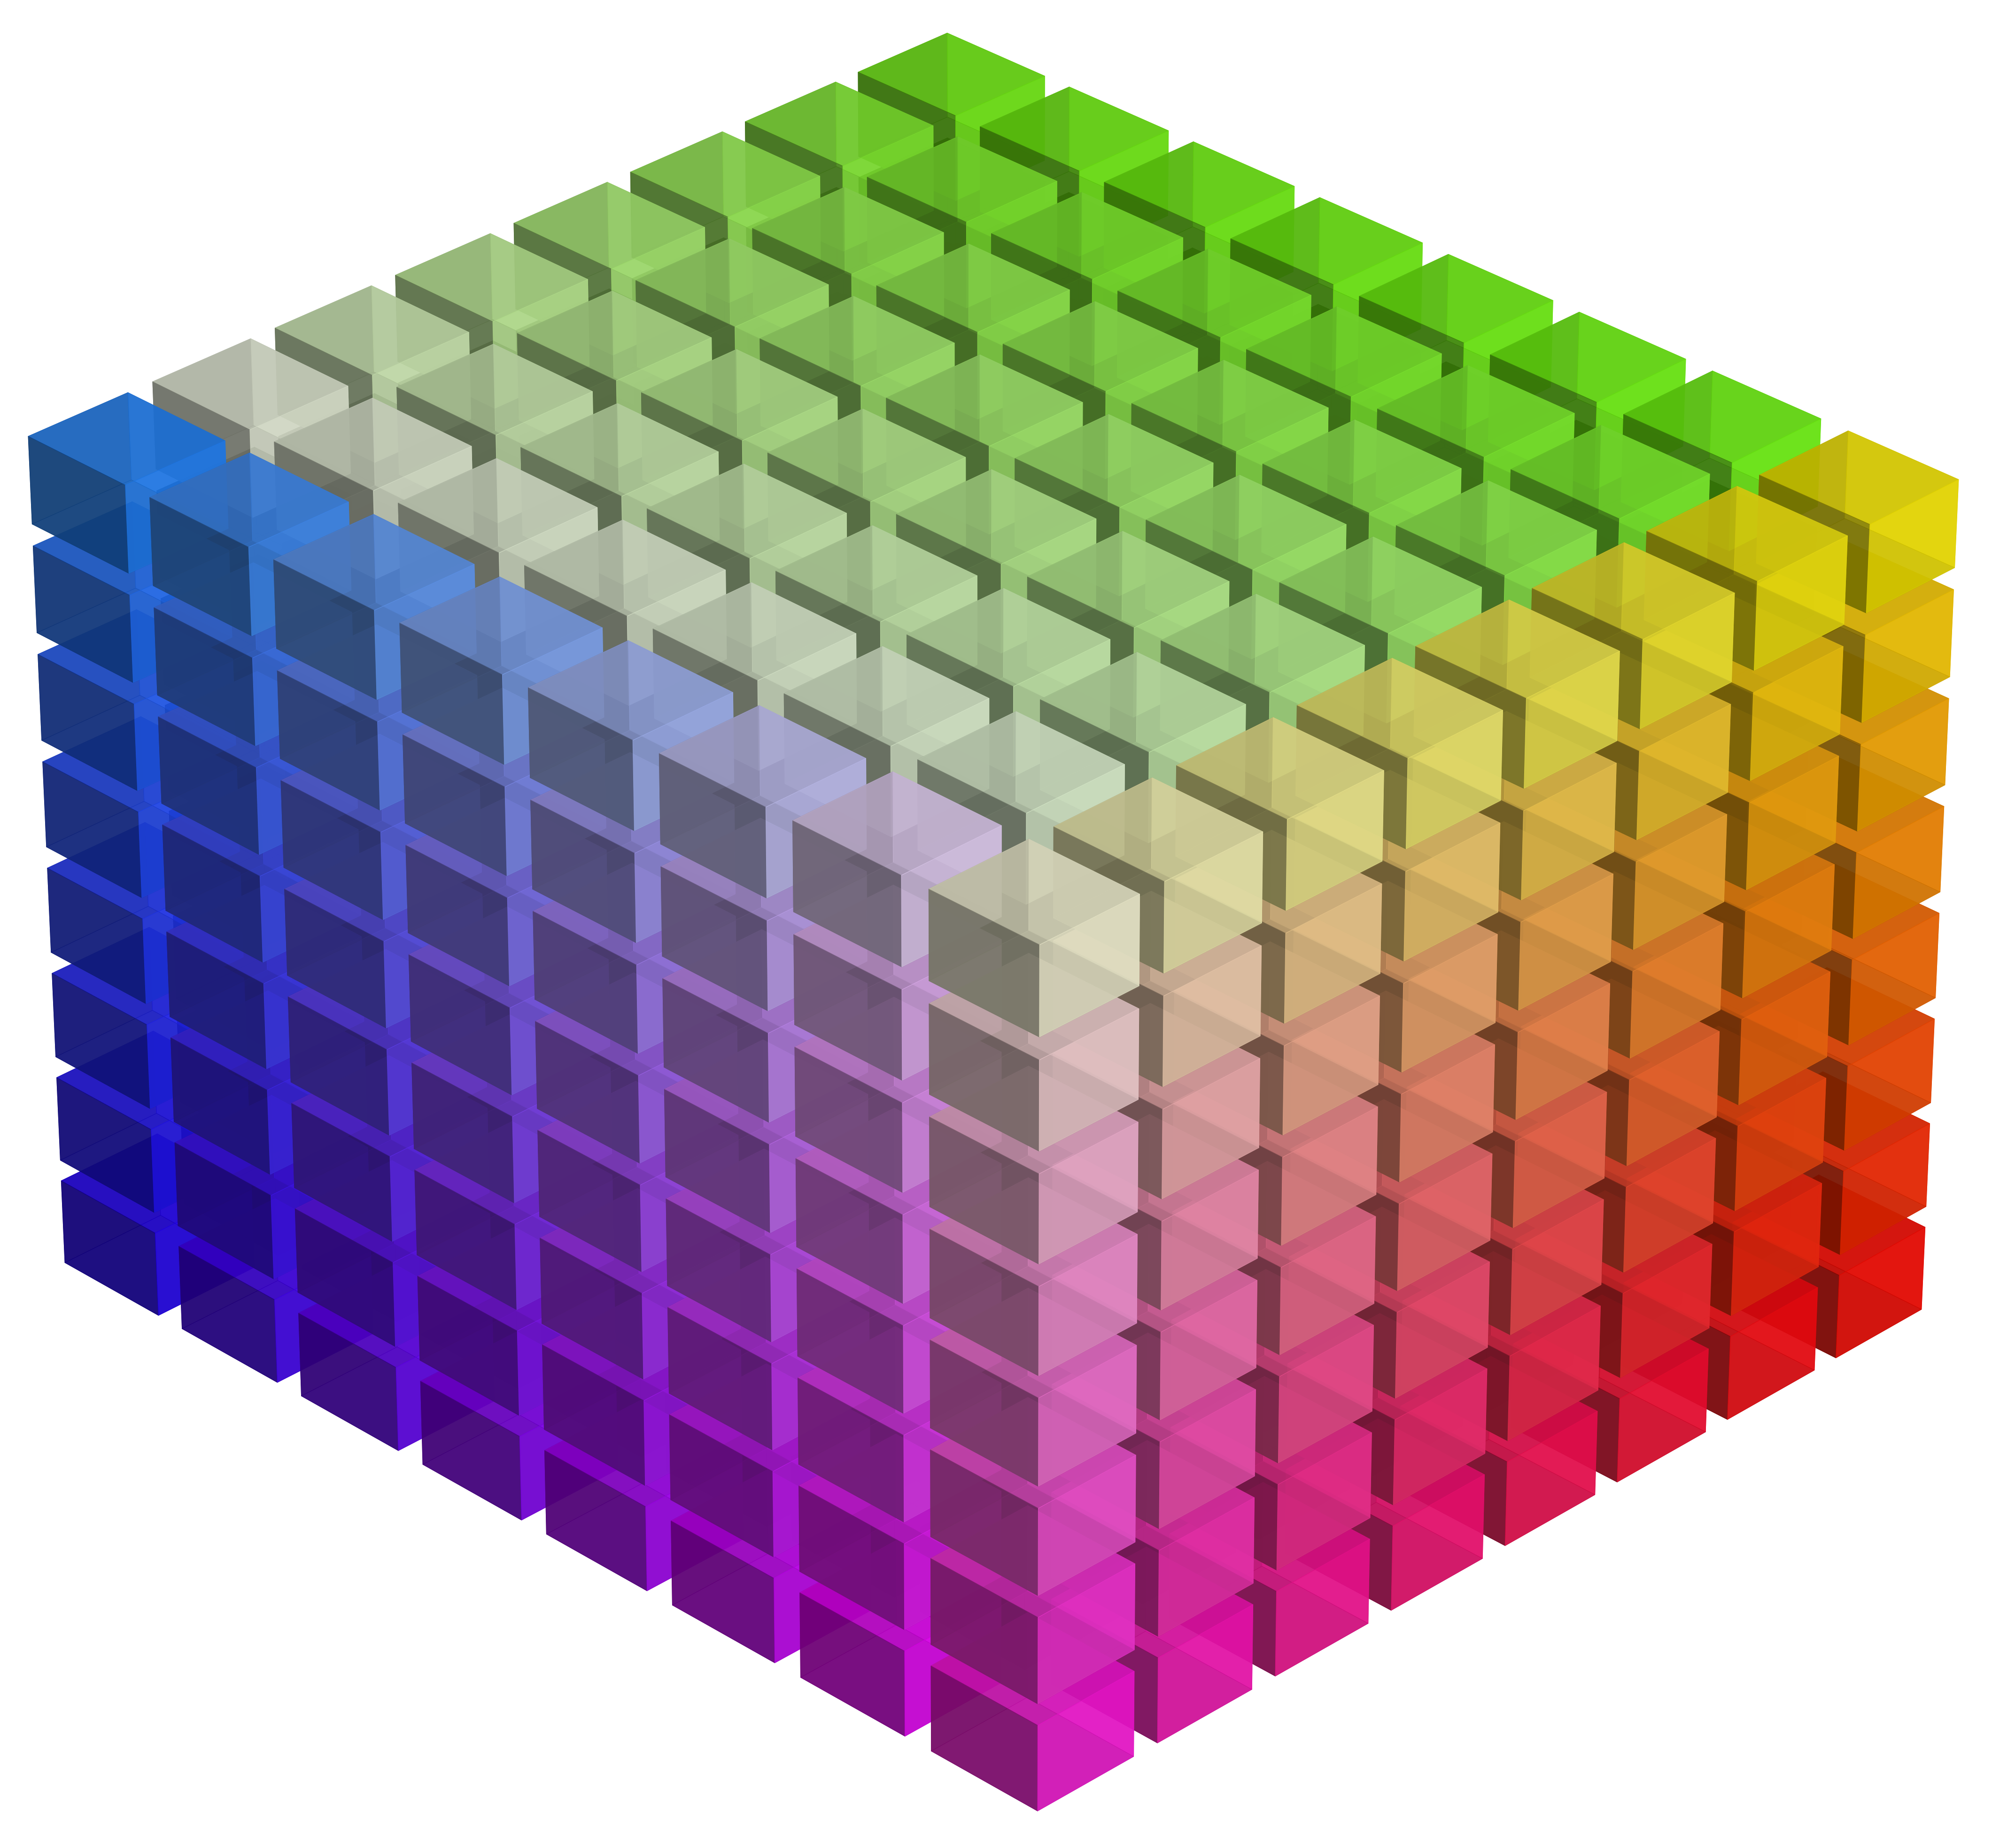
\includegraphics[width=12cm]{src/cry/cube.png}%
    \end{adjustbox}
\caption{This is not quite right, but you get the idea.}
\end{figure}

Now if we project this three dimensional object onto a flat surface, with our white top corner at the centre, we will have a 16x16 square
with 256 different colours:

\begin{figure}[H]
    \centering
    \begin{adjustbox}{width=4cm,center}
      \frame{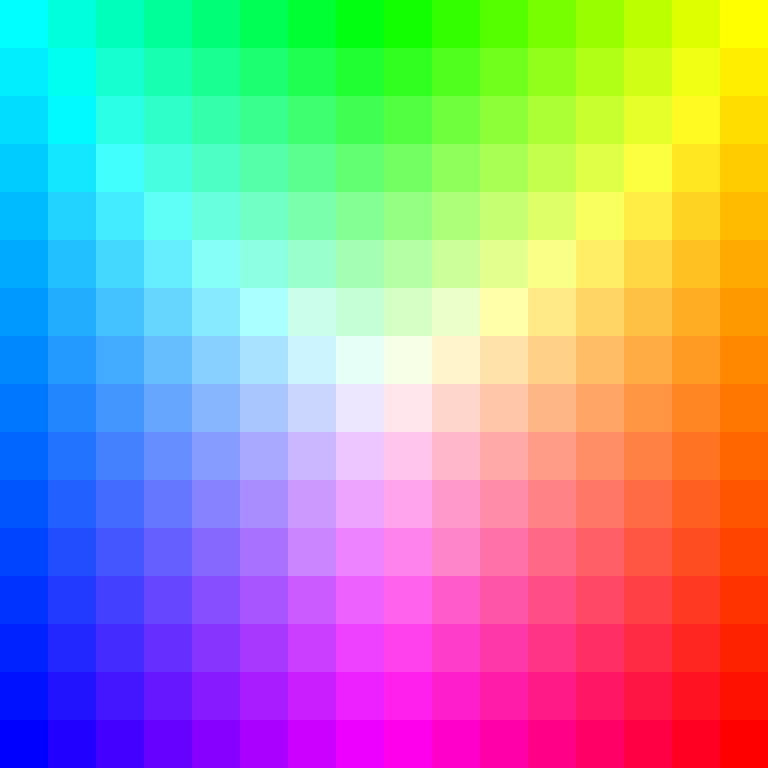
\includegraphics[width=12cm]{src/cry/2dcube.png}}%
    \end{adjustbox}
\caption{3d, but in 2d: it's the 1990s.}
\end{figure}

Since 256 is exactly the number of permutations in a single byte we have lit upon a use-case for the first of our two bytes.

\begin{figure}[H]
  {
    \setlength{\tabcolsep}{3.0pt}
    \setlength\cmidrulewidth{\lightrulewidth} % Make cmidrule = 
    \begin{adjustbox}{width=10cm,center}
      \begin{tikzpicture}
      \def\BACKGROUNDTWO{lightblue}
      \def\BACKGROUNDONE{lightgreen}
      \fill[\BACKGROUNDTWO] (0,0) rectangle ++ (1,1);
      \fill[\BACKGROUNDTWO] (1,0) rectangle ++ (1,1);
      \fill[\BACKGROUNDTWO] (2,0) rectangle ++ (1,1);
      \fill[\BACKGROUNDTWO] (3,0) rectangle ++ (1,1);
      \fill[\BACKGROUNDONE] (4,0) rectangle ++ (1,1);
      \fill[\BACKGROUNDONE] (5,0) rectangle ++ (1,1);
      \fill[\BACKGROUNDONE] (6,0) rectangle ++ (1,1);
      \fill[\BACKGROUNDONE] (7,0) rectangle ++ (1,1);
        \draw[step=1.0,gray,thin] (0,0) grid (1,1);
        \node[matrix of math nodes,anchor=south west,inner sep=0pt,
        nodes={draw,minimum size=1cm,anchor=center},
        column sep=-\pgflinewidth,row sep=-\pgflinewidth,font=\huge\ttfamily]
        {
          0 & 0  & 0 & 0 & 1 & 0 & 0 & 0 & 0 & 0  & 0 & 0 & 1 & 0 & 0 & 0\\
        };
      \end{tikzpicture}
    \end{adjustbox}
  }\caption{The first 8 bits now have a purpose. The first four are our X axis on the square, the second our Y axis.}
\end{figure}

This is all very nice, we have 256 colors going on and a whole other 8 bits to do something with. After thinking about it a bit, we don't
have too many options. In fact we have one option: use our extra 8 bits to vary each of our 256 colors in 256 different ways. We can make
this twiddle factor sound intelligent by calling it 'luminosity'. So depending on how much light we think is being cast on a surface with
the color in question we can use our final 8 bits to dial its brightness up or down.
\begin{figure}[H]
  {
    \setlength{\tabcolsep}{3.0pt}
    \setlength\cmidrulewidth{\lightrulewidth} % Make cmidrule = 
    \begin{adjustbox}{width=10cm,center}
      \begin{tikzpicture}
      \def\BACKGROUNDTWO{yellow}
      \fill[\BACKGROUNDTWO] (8,0) rectangle ++ (1,1);
      \fill[\BACKGROUNDTWO] (9,0) rectangle ++ (1,1);
      \fill[\BACKGROUNDTWO] (10,0) rectangle ++ (1,1);
      \fill[\BACKGROUNDTWO] (11,0) rectangle ++ (1,1);
      \fill[\BACKGROUNDTWO] (12,0) rectangle ++ (1,1);
      \fill[\BACKGROUNDTWO] (13,0) rectangle ++ (1,1);
      \fill[\BACKGROUNDTWO] (14,0) rectangle ++ (1,1);
      \fill[\BACKGROUNDTWO] (15,0) rectangle ++ (1,1);
        \draw[step=1.0,gray,thin] (0,0) grid (1,1);
        \node[matrix of math nodes,anchor=south west,inner sep=0pt,
        nodes={draw,minimum size=1cm,anchor=center},
        column sep=-\pgflinewidth,row sep=-\pgflinewidth,font=\huge\ttfamily]
        {
          0 & 0  & 0 & 0 & 1 & 0 & 0 & 0 & 0 & 0  & 0 & 0 & 1 & 0 & 0 & 0\\
        };
      \end{tikzpicture}
    \end{adjustbox}
  }\caption{The 8 bits representing the luminosity/intensity of the color chosen by the first 8 bits.}
\end{figure}

To get an idea of the effect this has in practice we can visualize our little color square repeating across a much
bigger square with ascending values of luminosity starting at 0 and ending at 255.
\begin{figure}[H]
    \centering
    \begin{adjustbox}{width=5cm,center}
      \frame{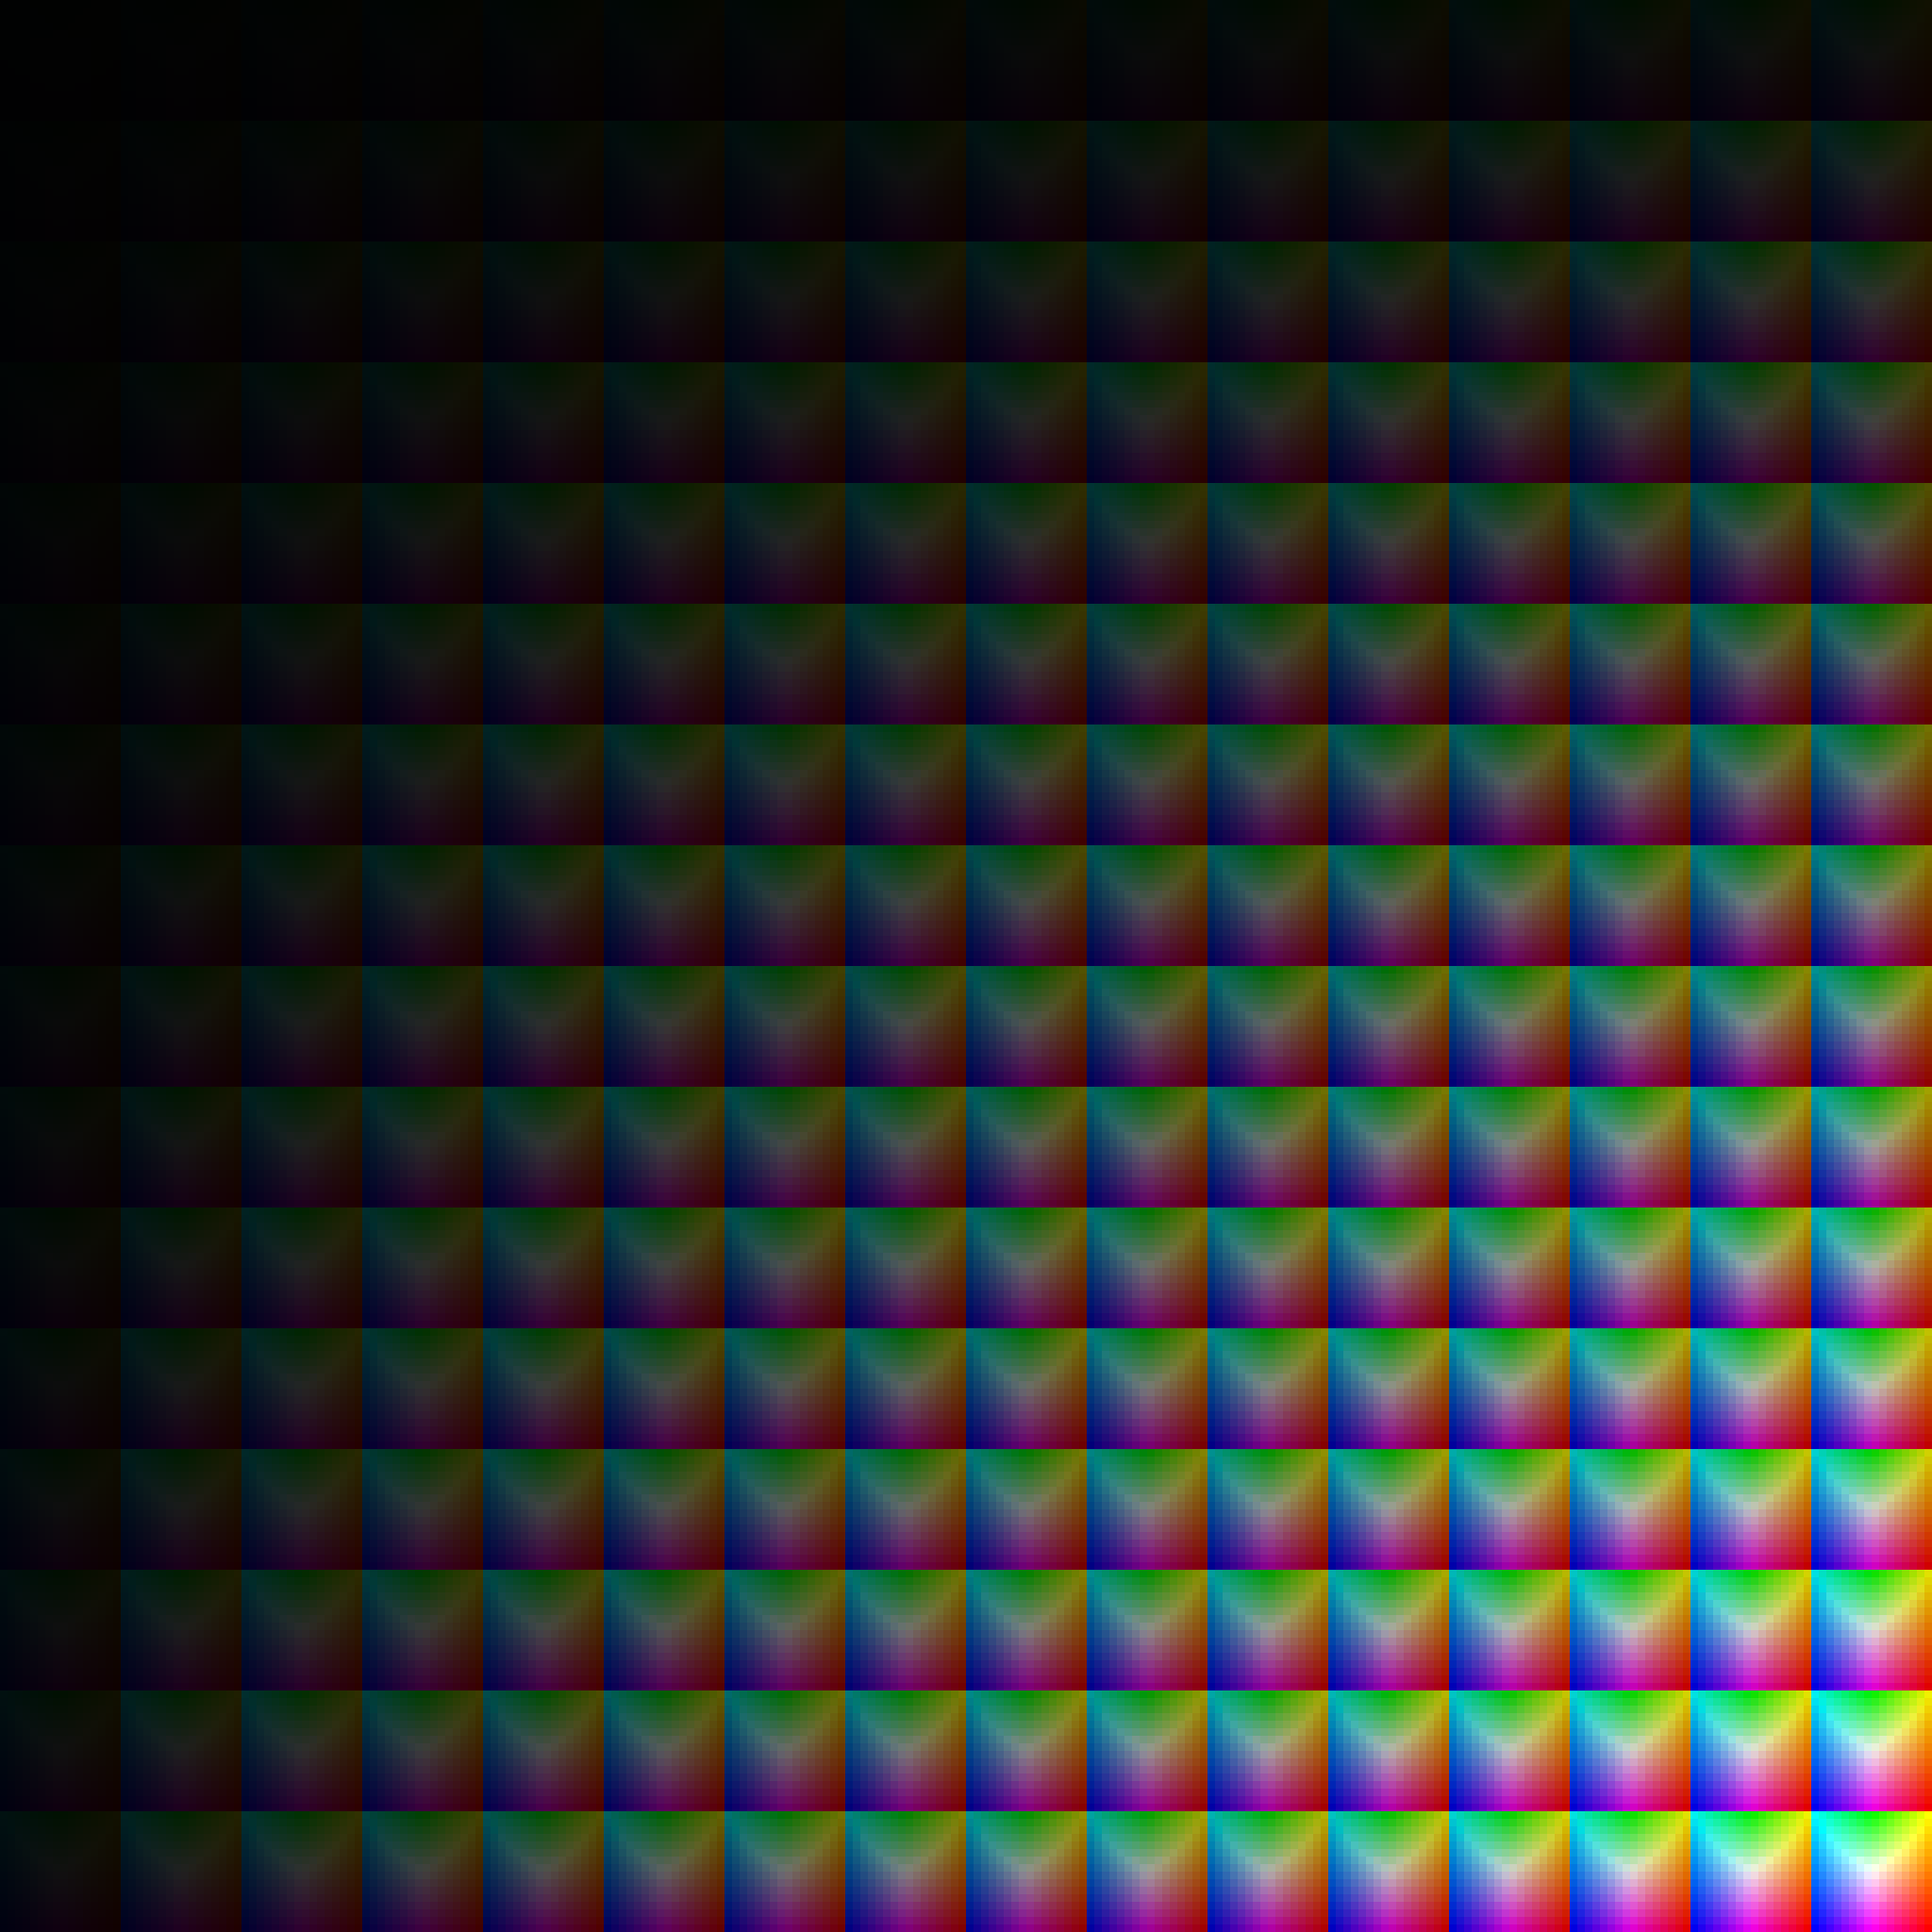
\includegraphics[width=12cm]{src/cry/2dcube-intensity.png}}%
    \end{adjustbox}
\caption{A big square with all our little squares in ascending luminosity.}
\end{figure}

That's a lot of dark. We better not wear shaded spectactles while playing games on this thing. Is there really 65,536 colors in there,
it seems like we have an awful lot of black going on. Let's try something and see what we get if we ignore all color values that appear
more than once.

\begin{figure}[H]
    \centering
    \begin{adjustbox}{width=5cm,center}
      \frame{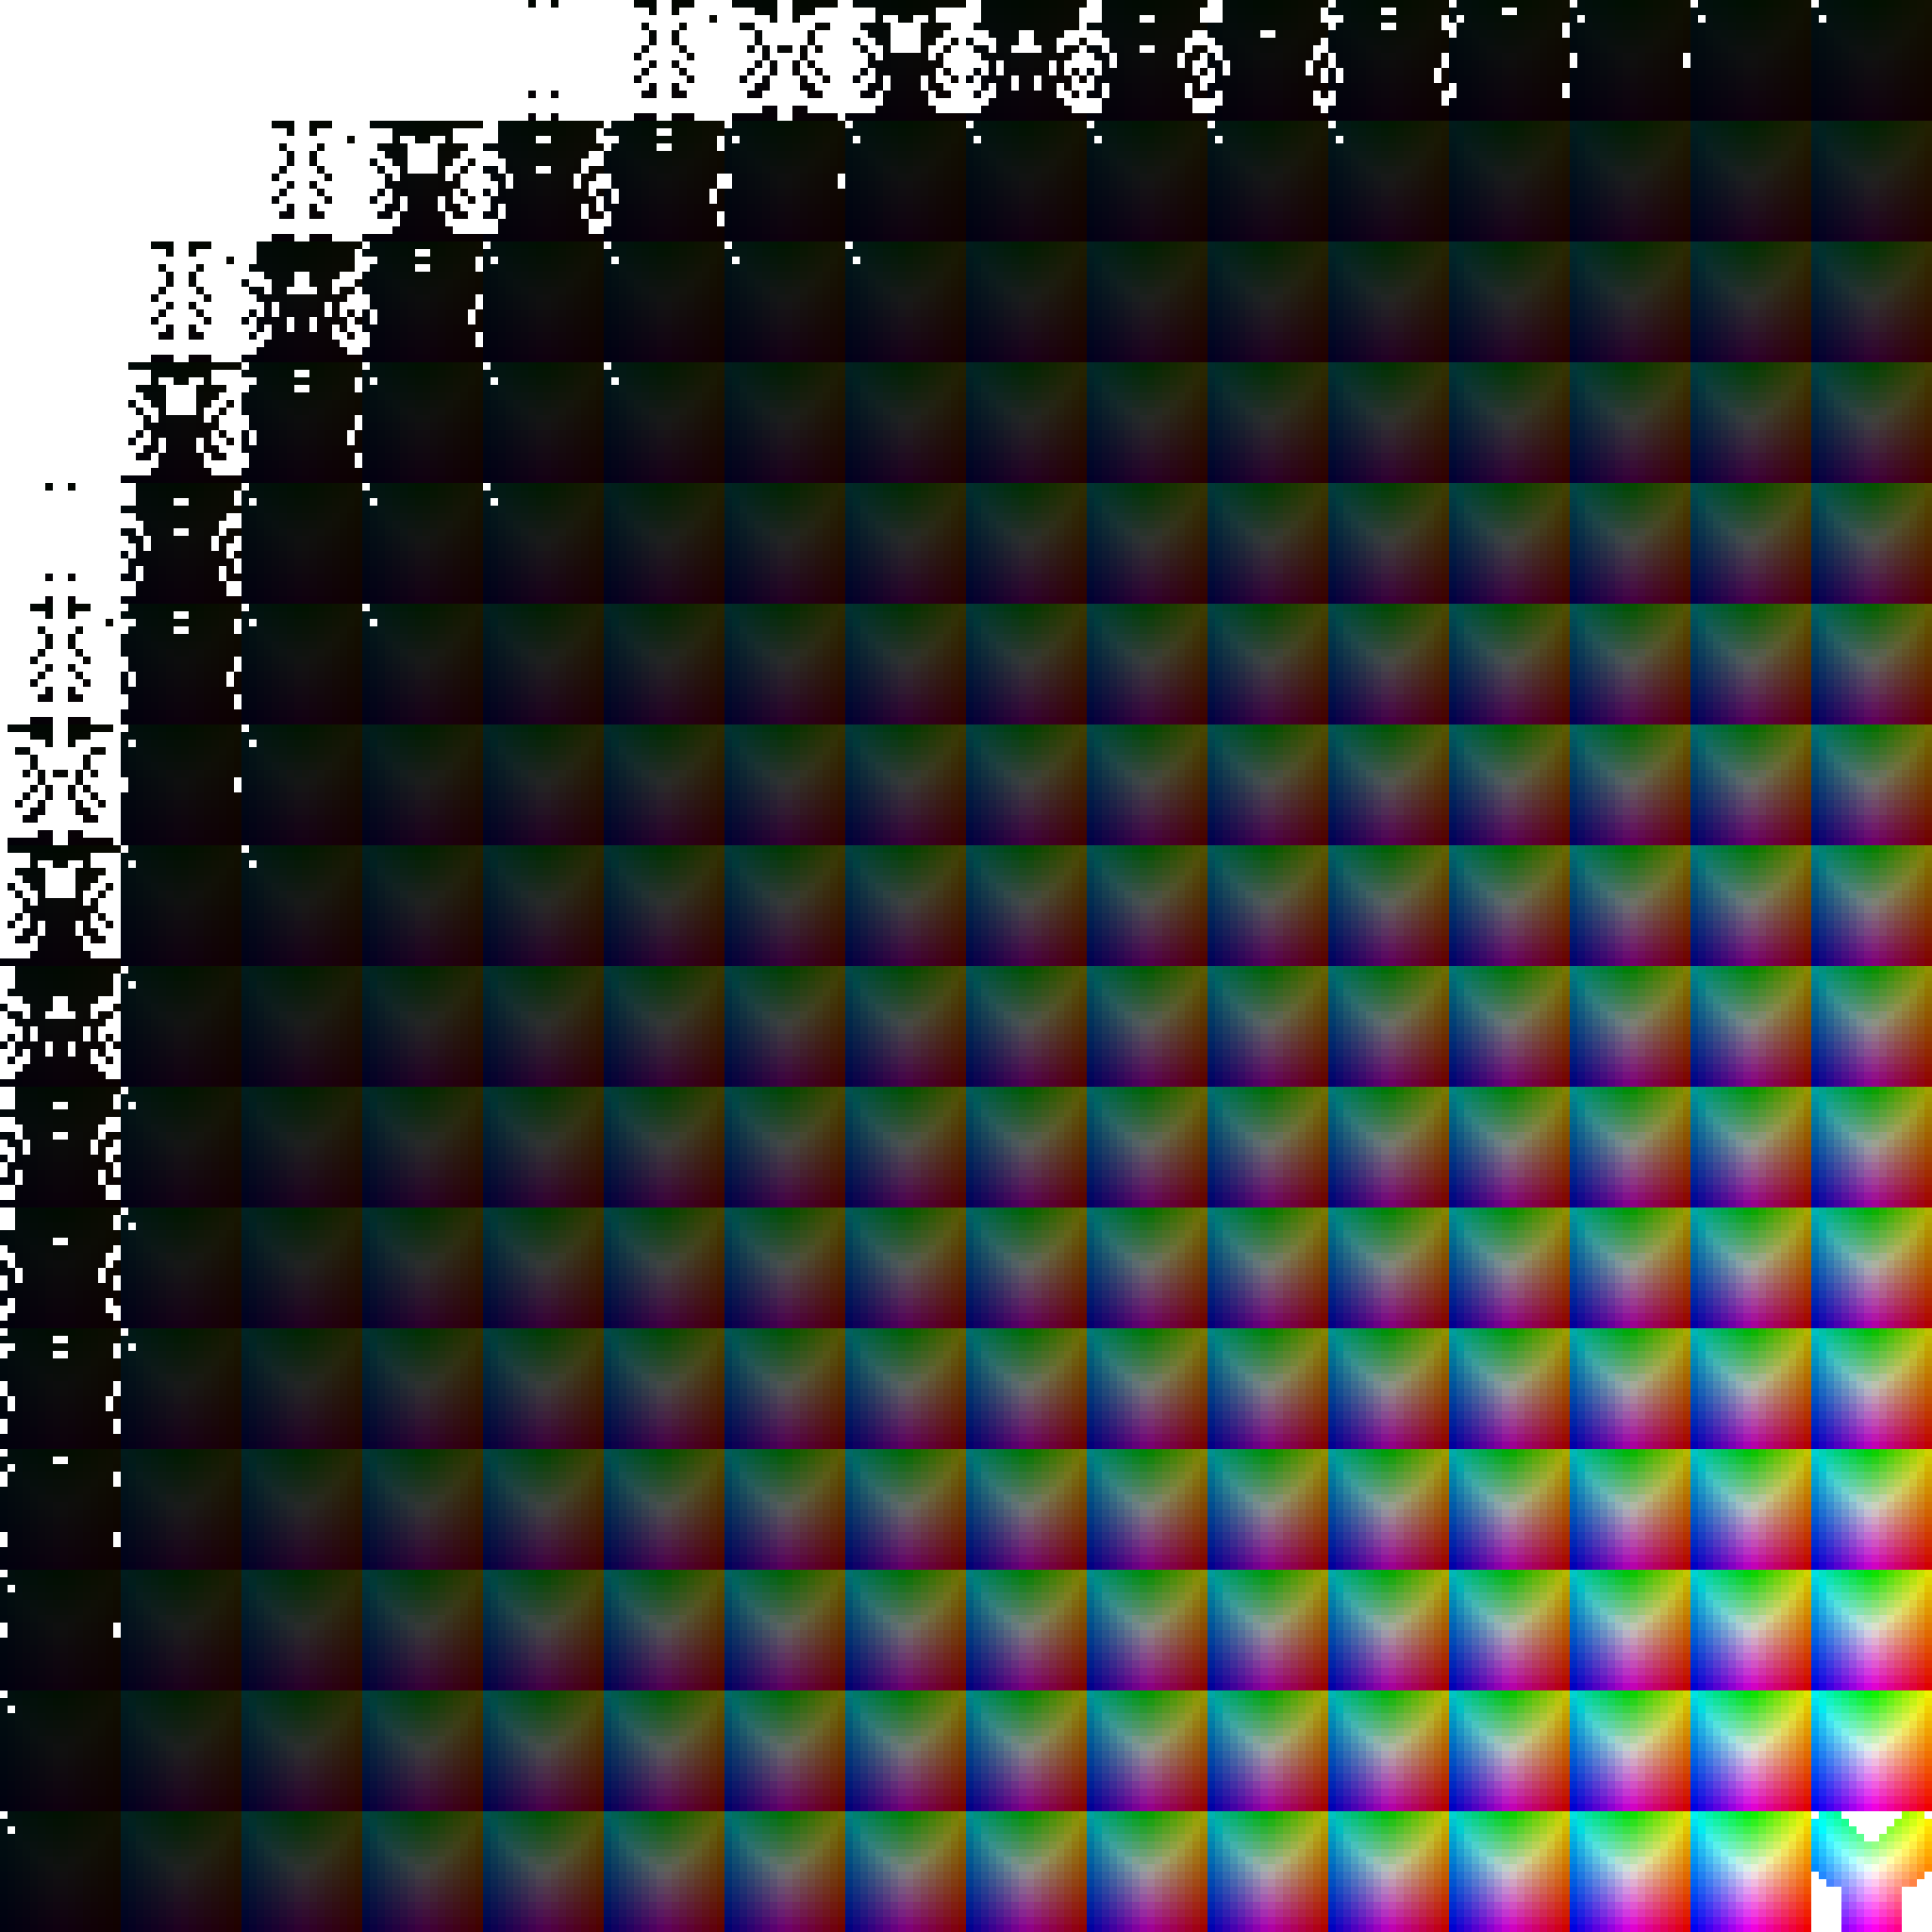
\includegraphics[width=12cm]{src/cry/2dcube-intensity-missing.png}}%
    \end{adjustbox}
\caption{Of course the 65,536 colors is a lie. I've counted them so you don't have to: there are 63,762 unique colours.}
\end{figure}

There are some strange little fractal shapes in the black stuff there. In the bottom right hand corner we can see that we eventually
run out of luminosity, our last little sqaure can only muster up 120 or so new colours.

\section*{the tempest files}
Now that we know what the bytes in a CRY image mean let's take a peek at the 6 image files in the Tempest 2000 sources to 
see what some of these bytes look like in practice. (Don't worry we'll be looking at all of these files in detail under one pretext
or another during the course of the rest of this book.) The seven image files are given slightly random, but very Minter-ish names: 
\icode{beasty3.cry}, \icode{beasty4.cry}, \icode{beasty5.cry}, \icode{beasty6.cry}, \icode{beasty7.cry} and  \icode{beasty8.cry}.


\begin{definition}[Claw Says\index{Claw Says}]
\setlength{\intextsep}{0pt}%
\setlength{\columnsep}{3pt}%
\begin{wrapfigure}{l}{0.12\textwidth}
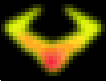
\includegraphics[width=\linewidth]{src/callout/claw.png} 
\end{wrapfigure}
\small
\textcolor{white}{
  Oh and let's not forget \icode{beasty8-xtra.cry}. This is a slightly larger version of \icode{beasty8.cry} included with the sources
  but for some reason is not used. There is also a story to tell about \icode{beasty3.cry} but we will come to that later.
}
\end{definition}

Remember there is nothing else in these files but the series of byte-pairs. There's no information about how big the image is or what
its dimensions are. It really is just a list. To cope with this fact the game hard-codes its own expectation that the
images are 320 pixels wide (i.e. the pixel width of the Jaguar's screen) and fixes the address that each image at will be loaded at.
It does this early on in the declaration of constants at the top of the main file containing all the game's code (\icode{yak.s}):

\begin{lstlisting}[escapechar=\%]
  pic          EQU $820000          ; beasty3.cry
  pic2         EQU pic+$1f400       ; beasty4.cry
  pic3         EQU pic2+$1f400      ; beasty5.cry
  pic4         EQU pic3+$25800      ; beasty6.cry
  pic5         EQU pic4+(640*128)   ; beasty7.cry
  pic6         EQU pic5+(640*200)   ; beasty8.cry
\end{lstlisting}

Each image has been loaded to a specific position in memory and the game is instructed exactly where each one is. While \icode{beasty3.cry}
is loaded to \icode{\$820000} (and assigned the variable name \icode{pic}), \icode{beasty4.cry} is loaded to the address 128,000 (\icode{\$1f400}) 
bytes after that and assigned the name \icode{pix2} because 128,000 bytes is how large \icode{beasty3.cry} is. You get the idea hopefully. 

As you can see in the above listing extract some of the images are larger than others so need more memory, but in all cases the assumption of treating every image as 320 pixels wide 
(640 bytes, since we have 2 bytes per pixel) holds.

Before passing on let's take a look at the contents of \icode{beasty7.cry}. 

\begin{figure}[H]
    \centering
    \begin{adjustbox}{width=8cm,center}
      \frame{
\includegraphics[width=12cm]{src/cry/beasty7.png}}%
    \end{adjustbox}
  \caption{\icode{beasty7.cry}, packed with goodness.}
\end{figure}

Looks great, you have to agree. We're in for some fun.

